\chapter{Ukázková webová aplikace}
V následující kapitole je představena ukázková webové aplikace, vyvinutá dle isomorfního přístupu, popsáného výše. Serverová i klientská část aplikace je tedy napsána v jazyce Javascipt. Tento přístup sjednocuje použitý jazyk a knihovny pro obě části aplikace a tím zjednodušuje a sbližuje implementaci celého systému moderní webové aplikace. Datová komunikace webového prohlížeče se serverem probíhá pomocí Websocketu. Server zasílá klientovi data ve formátu JSON (Javascript Object Notation \cite{json})). Ukázková webová aplikace představuje jednoduchou návštěvní knihu se základní funkcionalitou. Vytvořenou aplikaci můžeme zařadit mezi takzvané Rich Internet Applications \cite{ria}, tedy webové aplikace jejichž uživatelské prostředí se snaží uživateli poskytnout prostředky, které zná z běžných desktopových aplikací. Na rozdíl od tradičních webových aplikací není uživatelské prostředí tvořeno pouze základními prostředky jazyka HTML, ale hojně využivá javascriptové komponenty, implementované ve frameworku \textit{React} \cite{react}, který je zodpovědný za návrh a obsluhu interaktivního uživatelského rozhraní. Návod ke spuštění a instalaci ukázkové aplikace lze nalézt v přílohách této práce.

\vspace{3mm}
\begin{figure}[h]
\begin{centering}
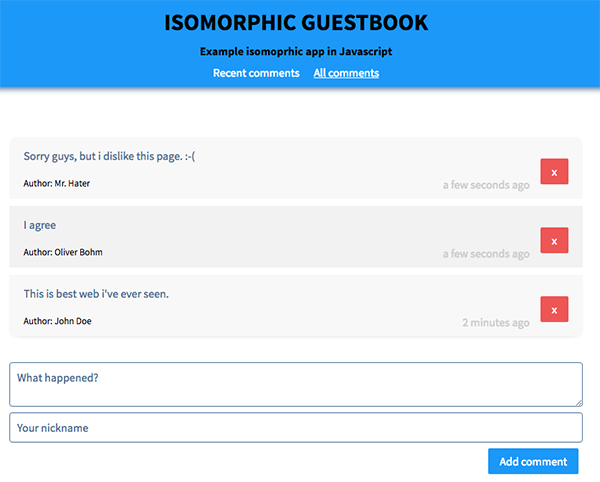
\includegraphics[scale=0.45]{obrazky/example_app}
\par\end{centering}
\caption{Ukázka vytvořené isomorfní aplikace.\label{fig:webpack}}
\end{figure}
\FloatBarrier

\section{Vybrané řešení}
Každá isomorfní aplikace většinou využívá připravené vývojové prostředí zvané devstack. Některé z nich jsou popsány v kapitole \hyperref[sec:devstacks]{4.6}. Jeho výběr úzce souvisí s knihovnami, které chce programátor využít. Autor používá vlastní devstack postavený nad starší verzí Este.js, který využívá React architekturu uživatelského rozhraní spolu s realtime NoSQL databází RethinkDB. Ten bude použit i v této práci.

\vspace{3mm}
\noindent \textbf{Použité technlogie}:
\begin{itemize}
\item React	JS – framework pro zobrazovací vrstvu,
\item React Router – isomorfní router,
\item Redux – správa aplikačního stavu,
\item RethinkDB	 – hlavní databáze,
\item Immutable.js – imutabilní datové struktury,
\item Express	– serverový framework pro node.js,
\item Socket.io – framework pro komunikaci mezi serverem a klientem,
\item Webpack – module bundler a nástroj pro build aplikace,
\item Superagent – univerzální knihovna pro práci s HTTP,
\item Stylus – CSS preprocesor.
\end{itemize}

\section{Hlavní principy implementace}
Popisovaná aplikace vznikla pro ilustraci několika principů moderního javascriptového návrhu. Jsou to především tyto.
\begin{itemize}
\item Isomorfní (univerzální) Javascript – viz kapitola \hyperref[sec:isomorphic]{4}.
\item Mobile first / Responsive design.
\item Offline ready.
\item Jednosměrný tok dat aplikací.
\item Asynchronní zpracování událostí s obsluhou chybových stavů.
\item Persistovaný globální aplikační stav.
\item Typový Dependency Injection kontejner.
\item Realtime komunikace a synchronizace.
\end{itemize}

Následující kapitola představí hlavní principy a návrhové vzory, které je vhodné použít při vývoji isomorfních webových aplikací. Tyto principy jsou výsledkem evoluce webových aplikací a jsou dnes běžnými metodami jejich návrhu v prostředí jazyka Javascript. Na následujících řádcích jsou některé z nich popsány detailněji.

\subsection{Offline-ready}
Celá aplikace je navržena tak, aby mohla běžet i v případě výpadku internetu. Toho je docíleno ukládáním dat webovou aplikací na straně uživatele a jejich odesílání na server dávkově v okamžiku obnovení spojení. Neexistuje žádná běžně používaná knihovna, kterou by bylo možné využívat pro tento účel, jedná se spíše o návrhový vzor, který popisuje práci s uživatelskými daty. Možnost pracovat s aplikací i ve stavu offline přinesly nové funkce webových prohlížečů definované standardem HTML5, především úložiště LocalStorage. Při použití vhodných nástrojů získáme možnost práce v offline režimu bez nároků na jakoukoli vlastní implementaci. Knihovna Redux, která je použita v ukázkové aplikaci pro správu dat, tento princip splňuje.

\subsection{Mobile-first / Responsive design}
Dnešní webové aplikace musí být vyvíjeny s ohledem na existenci obrovské škály rozlišení webových prohlížečů. Aplikace musí být schopná adaptace na velikost zobrazovací plochy koncových zařízení a bezchybně se zobrazit na běžných počítačích, tabletech nebo mobilních telefonech. Moderní notebooky s velmi vysokým rozlišením je také nutné zohlednit. Tento přístup se nazývá responzivní design a je zpravidla realizován několika hlavními způsoby. Jedním z nich je vytvoření zcela odděleného mobilního webu, na který je pak uživatel přesměrován, přichází-li z mobilního zařízení. Nasazení odděleného mobilní webu je vhodné především pro velmi složité layouty, jejichž adaptace na nízké rozlišení by byla náročná. Druhým, v současnosti doporučovaným přístupem, je automatická adaptace webové stránky na dostupné rozlišení. Většinou to znamená nutnost nastylování webu nejméně pro tři základní zařízení, desktop, tablet a mobilní telefon. Základním konstruktem pro implementaci adaptivního stylování jsou \textit{media queries} v jazyce CSS, pomocí nichž lze definovat stylopis pouze pro určité rozlišení. Samotný responzivní přístup není možné plně automatizovat a je plně v konpetenci programátora uživatelského rozhraní. Existuje však mnoho CSS frameworků, které dokážou vývoj usnadnit. Vhodné je také použití některého z CSS preprocesorů, které vylepšují syntaxi CSS přidáním možnosti zanořování deklarací nebo možnosti definovice vlastních proměnných. Mezi nejpoužívanější tři z nich patří Less, Sass a Stylus. Ukázková aplikace využívá preprocesor Stylus \cite{stylus}, především kvůli osobním preferencím autora práce.

\subsection{Jeden stav aplikace}
Každá isomorfní aplikace je hluboce založená na jejím stavu, každá změna v aplikaci je realizována na základě změny tohoto stavu. V isomorfních aplikacích stav určuje celý vzhled aplikace, obsahuje veškerá data i stav všech existujících DOM elementů. Je doporučováno ukládat kompletní stav aplikace do jediného javascriptového objektu. Ten lze následně ukládat na straně uživatele nebo ho propagovat pomocí Websocketu do všech aktuálně otevřených oken jednoho uživatele. Tento přístup zjednodušuje implementaci webových aplikací, není totiž nutné počítat s různými stavy aplikace v době odeslání požadavku na server. Ukládání stavu na straně uživatele, například pomocí HTML5 Local storage, zase umožňuje obnovení celé aplikace například v případě pádu webového prohlížeče. Správa stavu aplikace, jeho ukládání, provádění změn, nebo jeho obnova, je v ukázkové aplikaci řešena pomocí knihovny Redux. Tato knihovna je implementací návrhového vzoru Flux, který popisuje práci se stavy (viz. \hyperref[sec:flux]{4.4.6}). Flux byl představen společností Facebook v roce 2015, nutnost sjednotit správu aplikačních stavů vznikla při programování známé sociální sítě. Existuje mnoho implementaci tohoto návrhového vzoru, Redux je v současnosti jeho preferovanou implementací. Je také plně kompatibilní s isomorfním přístupem, proto je využit i v ukázkové aplikaci \cite{redux}. 

\vspace{3mm}
\begin{figure}[h]
\begin{centering}
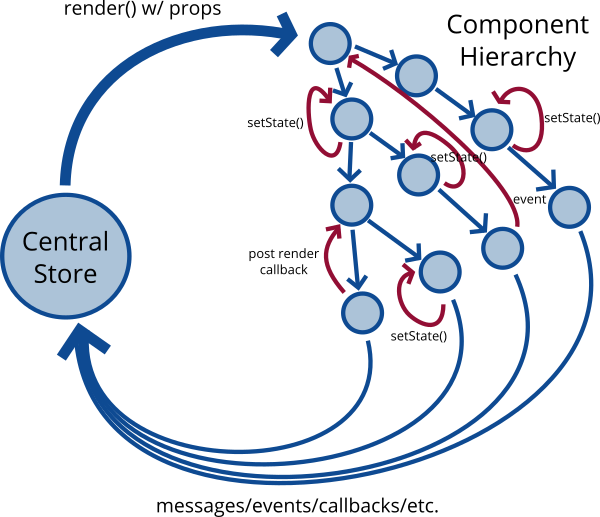
\includegraphics[scale=0.5]{obrazky/central_store}
\par\end{centering}
\caption{Diagram správy stavu aplikace pomocí frameworků React a Redux \cite{react_best_practices}} \label{fig:central_store}
\end{figure}
\FloatBarrier

\subsection{Jednosměrný tok dat}
Aplikace je vždy kompletně překreslena z virtuálního DOM při každé změně jejího stavu. Framework React používá jednosměrný tok dat – od vlastníka do vlastněné komponenty. Tento proces se opakuje rekurzivně dokud nejsou data aktualizována na všech místech. Tímto je zajištěna aktuálnost všech dat isomorfní webové aplikace. Komponenty přijímají data pouze v okamžiku vykreslování. Když se data změní, framework zajístí předání aktuálních dat a komponenta se vykreslí znovu. Tento princip si klade za cíl zjednodušit předávání dat v aplikaci \cite{react}.

\vspace{3mm}
\begin{figure}[h]
\begin{centering}
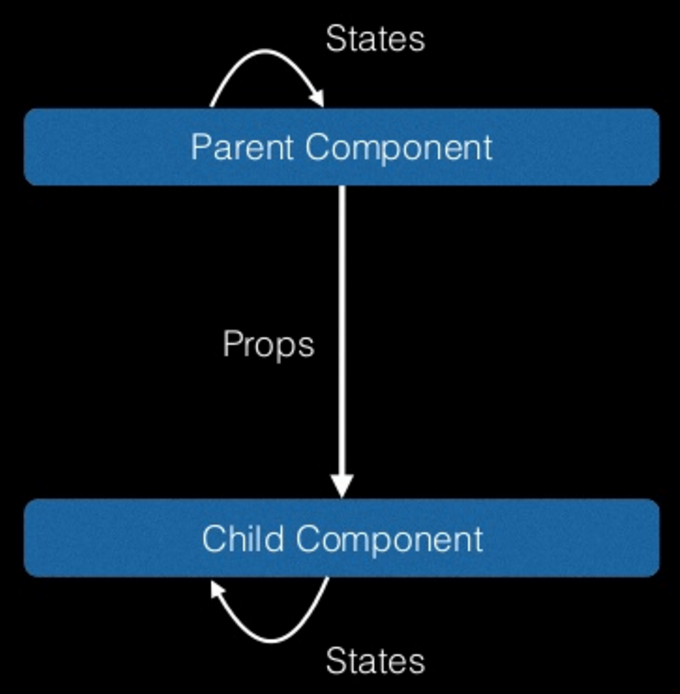
\includegraphics[scale=0.3]{obrazky/oneway_dataflow}
\par\end{centering}
\caption{Diagram jednosměrného toku data v React \cite{react} \label{fig:onewaydataflow}}
\end{figure}
\FloatBarrier

\subsection{Realtime komunikace a synchronizace}
Celá aplikace je velmi interaktivní a podporuje realtime komunikaci s databází. Přidání nové položky nebo její změna se okamžitě projeví u všech připojených uživatelů, bez nutnosti znovu načítat stránku. Doručení nových dat do webových prohlížečů je realizováno pomocí Websocketu, změny není nutné periodicky ověřovat, server změnu doručí sám, jakmile k ní dojde. Synchronizace stavu aplikace probíhá nejen mezi různými uživateli, ale pochopitelně také mezi více okny jednoho uživatele. Rychlé propagaci nových dat také pomáhá použitá databáze RethinkDB, která pomocí triggerů umožňuje notifikovat webovou aplikaci o změně uložených dat. Ta potom provede aktualizaci jejich zobrazení \cite{rethinkdb}. Použití této databáze je podrobněji popsáno v kapitole \hyperref[sec:rethinkdb]{5.3.7}. 

\section{Použité technologie}
Následující kapitola shrnuje technologie a související knihovny, které byly použity v ukázkové isomorfní webové aplikaci. U každé k knihoven je uveden její účel spolu se souvisejícím příkladem zdrojového kódu. Použitý kód pochází přímo z implementace ukázkové webové aplikace.

\subsection{node.js}
Node.js je základní předpoklad isomorfního přístupu, umožňuje zpracovávat javascriptový kód na serveru, a tím přináší serverové vykreslování šablon, které řeší mnohé problémy typických jednostránkových webových aplikací. To je popsáno v kapitole \hyperref[sec:node_js]{2.4}. Spolu s node.js se v ukázkové aplikaci používá také balíčkovací systém NPM, který řeší správu závislostí a spouštění obslužných skriptů vyvíjené aplikace \cite{nodejs} \cite{npm}.

\subsection{express}
Minimalistický framework Express je de facto standardizovaným serverovým frameworkem pro node.js. Ulehčuje definování aplikačních rozhraní, práci s databází a podobně. U isomorfních aplikací se především používá jako datové API. Je také plně kompatibilní s knihovnou React, kterou využívá při serverovém vykreslování šablon \cite{express}. Následující ukázka kódu popisuje definici dvou vstupních bodů API a příklad implementace server-side renderingu.

\begin{lstlisting}[language=Javascript,caption={Ukázka konfigurace serverového JS frameworku Express}]
var express=require('express');
var app = express();

app.get('/api/comments', function(req, res) {
  /* zpracovaní požadavku a vrácení dat */
});

app.post('/api/comments', function(req, res) {
    /* zpracovaní požadavku a vrácení dat */
});

app.get(['/'], function(req, res) { // server-side rendering
  /* Use React Router */
  var ReactRouter = require('react-router');
  var match = ReactRouter.match;
  var routes = require('./public/routes.js').routes

  match({routes: routes, location: req.url}, function(error, redirectLocation, renderProps) {
    /* vykreslení celé React aplikace a jeji vrácení jako čisté HTML */
  });
});
\end{lstlisting}

\subsection{React}
Framework React je knihovna pro tvorbu uživatelského rozhraní od společnosti Facebook. Je podrobně popsána v kapitolách \hyperref[sec:react]{2.8.3} a \hyperref[sec:react_isomoprhic]{4.4.5}.

Díky svému úzkému zaměření na vykreslování HTML, je vhodná pro použití v isomorfních aplikacích, protože bezproblémově běží v prohlížeči i na serveru \cite{react}. 

\subsubsection{Hlavní komponenta aplikace}
Následuje ukázka kódu hlavní React komponenty, která definuje celou webovou aplikaci. Je vidět použití komponent Header a Footer, reprezentujících společné části layoutu – hlavičku a patičku. Datové entity (komentáře) jsou hlavní komponentě předány pomocí props (viz \hyperref[sec:react_props]{2.4}). Pod komentáři se nachází formulář pro přidání nového komentáře. Tato komponenta představuje nejvyšší uzel stromu komponent, její změna tedy vyvolá překreslení celé webové aplikace. Tato ukázka představuje implementaci této komponenty v ukázkové webové aplikaci.
\begin{lstlisting}[language=Javascript,caption={Render metoda hlavní React komponenty GuestbookApp}]
  render() {
    let actions = { 
      editEvent: this.props.editEvent, 
      deleteEvent: this.props.deleteEvent
    };
    return (
      <div id="GuestbookApp">
        <Header/>
        <AsyncBar isWorking={this.props.isWorking} error={this.props.error} />
        {this.props.comments}
        <section className='container addCommentForm'>
          <CommentInput onSubmit={this.props.addEvent} userId={this.props.userId} textLabel='What happened?' authorLabel='Your nickname' valueLabel='Rating' />
        </section>
        <Footer/>
      </div>
    );
  }
\end{lstlisting}

\subsubsection{Datové komponenty}
Další skupinu komponent tvoří ty, která zobrazují data. Jedná se většinou o datové kontejnery, které zobrazují kolekce, nebo o jednoduché HTML komponenty vizualizující nějaká data. Syntaxe JSX, která kombinuje HTML a Javascript, dovoluje zobrazovat datové entity pomocí funkce \textit{map()}, která dostává definici datové komponenty jako argument. To umožňuje psát kratší a čitelnější kód, jak je vidět na příkladu níže. Na něm je také patrné řešení zástupného textu, pokud neexistují žádné komentáře.
\begin{lstlisting}[language=Javascript,caption={Render metoda datové komponenty CommentList pro zobrazení komentářů}]
render(){
   let list;
    if (comments.length > 0) {
      list = comments.map((event, key) =>
        <CommentItem key={key} row={key} id={event.id} editable={editable} event={event} {...actions} />
      );
    } else {
      list = <p>No comments!</p>;
    }
    return (
      <section className='container'>
        <div className='commentList'>
          <ul>
            {list}
          </ul>
        </div>
      </section>
    );
}
\end{lstlisting}

Na této ukázce kódu je vidět implementace jednoduché datové komponenty, která zobrazuje předaná data. Tvoří HTML reprezentaci některé z použitých datových entit, v našem případě se jedná o komentář. Ukázka také demonstruje princip jednotné zodpovědnosti, aby datová komponenta nemusela řešit mazání komentáře, dostává celou logiku nezbytnou pro mazání zvenčí jako property – \textit{ \{del\}} v ukázce (viz. \hyperref[sec:react_props]{2.4}).
\begin{lstlisting}[language=Javascript,caption={Render metoda komponenty CommentItem reprezentující komentář}]
render(){
  return (
     <div className='commentItem'>
          <p className='title'>
            {comment.text}
          </p><br/>
          {del}<br/>
          <p className='author'>
             Author: {comment.author}
          </p>
          <p className='created'>{moment(modified).fromNow()}</p>
     </div>
     );
}
\end{lstlisting}


\subsubsection{React router}
Velmi důležitou součástí každé webové aplikace je router, u isomorfních je nutné používat jeden router pro webový prohlížeč a druhý pro server. Díky možnostem moderního javascriptu však můžeme deklaraci routovacích pravidel extrahovat do vlastního souboru, který lze použít v obou routerech. V aplikaci se využívá React-router, jednotlivá pravidla se zapisují pomocí syntaxe JSX \cite{react_router}.
\begin{lstlisting}[language=Javascript,caption={Deklarace routovacích pravidel pomocí nástroje React-router}]
    <Route path='/' component={GuestbookApp}>
       <IndexRoute components={{comments: RecentComments}} />
       <Route path='all-comments' components={{comments: AllComments}} />
    </Route>
\end{lstlisting}

Knihovna React-router také poskytuje nástroje pro generování HTML odkazů na základě routovacích pravidel. Díky tomu není při tvorbě odkazů nutné používat HTML tag \textbf{a} a přemýšlet nad správným URL \cite{react_router}. Syntaxe je zřejmá z následující ukázky. 
\begin{lstlisting}[language=Javascript,caption={Využití generování HTML odkazů pomocí nástroje React-router}]
<ul>
	<li><Link to="/" activeStyle={{fontWeight: 'bold'}} onlyActiveOnIndex>Comments</Link></li>
	<li><Link to="/another-page" activeStyle={{fontWeight: 'bold'}}>Another Page</Link></li>
</ul>
\end{lstlisting}

\subsubsection{Čtení formulářových dat}
React také velmi usnadňuje tvorbu formulářů, pomáhá při jejich ověřování a řeší také odesílaní vstupních dat. Většinou se pro navěšování událostí na formulářové prvky používají klasické HTML atributy \textit{onClick}, \textit{onChange} a jim podobné. React ale nepoužívá oboustranný data binding \footnote{Data - binding poskytuje flexibilní mechanismus pro synchronizaci dat a uživatelského rozhraní.}, proto je nutné načíst formulářová data ručně \cite{react}. Tlačítko, které většinou řídí odesílání dat, musí získat přístup k HTML inputům, které drží data. Každá změna jakéhokoliv formulářového prvku fakticky vytváří nový stav související React komponenty, která ho zobrazuje. Často se proto používají takzvané \uv{watcher funkce}, které reagují na změnu formulářového prvku a jeho novou hodnotu ihned propagují do stavu příslušné komponenty. To je použito i v ukázkové aplikaci, implementace tohoto řešení je vidět na ukázce níže.
 
\begin{lstlisting}[language=Javascript,caption={Ukázka propagace hodnot formulářových polí do stavu React komponenty}]
  handleAuthorChange(e){ // handleTextChange je velmi podobná metoda
    this.setState({ author: e.target.value });
  }
  
  render(){
  ...  
  <textarea ... onChange={::this.handleTextChange}></textarea>
  <input ... onChange={::this.handleAuthorChange}/>
  ...
  }
\end{lstlisting}

\subsubsection{Server-side rendering}
Jednou se stěžejních technik isomorfního přístupu je server-side rendering, detailně popsaný v kapitole \hyperref[sec:server_side_rendering]{4.1.6}. Tento přístup umožňuje vygenerovat prvotní stav jednostránkové isomorfní aplikace na serveru pomocí node.js, což velmi urychluje načítání jednostránkových aplikací a tento prvotní stav se také zobrazí vyhledávacím robotům nebo uživatelům s vypnutým Javascriptem. Následující ukázka je demonstrací serverového vykreslení prvotního stavu webové aplikace.
\begin{lstlisting}[language=Javascript,caption={Ukázka propagování stavu aplikace ze serveru do prohlížeče }]
export function handleRender(req, res) {  
    // vytvoříme nový Redux store
    const store = createStore(rootReducer, {comments: initialComments, userId: 'baseUser'}); // userId bude vytvořeno až v prohlížeči

    // vykreslíme celou aplikaci do textu
    const html = React.renderToString(
      <Provider store={store}>
        {() => <GuestbookApp />}
      </Provider>
    );

    // odešleme vykreslenou aplikaci spolu s počátečním stavem do prohlížeče
    res.render('index', { html: html, initialState: JSON.stringify(store.getState()) });
}
\end{lstlisting}

Celá React aplikace se nejprve vykreslí do HTML pomocí serverového Javascriptu a spolu s počátečním stavem aplikace je odeslána do webového prohlížeče. Počáteční stav aplikace, který reprezentuje Redux store je serializován a uložen do proměnné \textit{window.\_\_INITIAL\_STATE\_\_}, ze které je pak store na klientské straně opět obnoven a celá aplikace spuštěna we webovém prohlížeči.

\begin{lstlisting}[language=Javascript,caption={Ukázka získaní počátečního stavu aplikace z webového prohlížeče}]
// získáme počáteční stav z globální promenně vygenerované serverem
let initialState = window.__INITIAL_STATE__;
const createStoreWithMiddleware = applyMiddleware(  
  thunkMiddleware,
  loggerMiddleware
)(createStore);

// vytvoříme z počátečního stavu Redux store
const store = createStoreWithMiddleware(actionReducers, initialState);

// překreslíme aplikaci v prohlížeči
React.render(  
  <Provider store={store}>
    {() => <GuestbookApp />}
  </Provider>,
  document.getElementById('app')
);

\end{lstlisting}
Serverové vykreslování nefunguje pouze pro úvodní stránku webové aplikace, server rozumí definicím klientských routovacích pravidel, takže načtení prvotního stavu a spuštění celé aplikace je možné na jakékoliv veřejně dostupné URL. Především díky tomu není indexování isomorfních aplikací žádný problém.

\subsection{Redux}
Isomorfní aplikace také přinesly novou architekturu zacházení s daty, známou jako Flux. Tento způsob práce s daty webové aplikace představila společnost Facebook a pojednává o něm kapitola \hyperref[sec:flux]{4.4.6}. Redux je v současné době preferovaná implementace tohoto návrhového vzoru. Při práci s Reduxem se používají tři základní konstrukce: \textit{store}, \textit{akce} a \textit{reducer}, který je mírně upravenou implementací dispatcheru popisovaného vzorem Flux \cite{redux}.

\subsubsection{Store}
Store tvoří \uv{srdce} celé isomorfní webové aplikace, jsou v něm uloženy veškerá data, stavy React komponent a některé další objekty. Store jako takový tvoří stav aplikace a existuje vždy právě jeden. Vytvořit ho pomocí nástroje Redux lze takto \cite{redux}:
\begin{lstlisting}[language=Javascript]
var store = Redux.createStore(reducer);
\end{lstlisting}

\vspace{3mm}
\noindent Store poskytuje tyto 3 základní metody, které řeší veškeré nezbytné operace \cite{redux}.
\begin{itemize}
\item store.getState() - vrací naše data (state)
\item store.subscribe(callback) – navěšení listener funkce na změnu store
\item store.dispatch(akce) – provádíme akci, která změní data ve store uložená
\end{itemize}

\subsubsection{Akce}
Pokud chceme provést změnu ve store (nebo obecně v aplikaci), je nutné tuto změnu realizovat pomocí jednoduchého objektu zvaného akce. Objekt akce má jediný povinný atribut zvaný \textit{type}, který slouží pro identifikaci akce reducerem při jejím vyhodnocování (viz níže). Jakékoliv další atributy jsou volitelné pro každou akci. Ta ale musí být jednoznačně identifikovatelná a musí obsahovat všechna data nutná k jejímu provedení.

\pagebreak
\noindent Příklady tří akcí v ukázkové webové aplikaci:
\begin{lstlisting}[language=Javascript, caption={Ukázka několika Redux akcí}]
{
    type: "ADD_COMMENT",
    text: "I really love your website!",
    author: "John Doe"
}
{
    type: "REMOVE_COMMENT",
    id: 15
}
{
    type: "REMOVE_ALL"
}
\end{lstlisting}

Tento objekt popisuje změnu dat, která bude provedena. Akcí popsaná změna se realizuje pomocí metody \textit{dispatch(akce)} nad store, která vyžaduje danou akci jako svůj jediný argument.

\begin{lstlisting}[language=Javascript, caption={Ukázka volání akce na Redux store}]
store.dispatch({ type: 'ADD_COMMENT', text: "I really love your website!", author: "John Doe" });
\end{lstlisting}

\subsubsection{Reducer}
Poslední nezbytnou součástí Reduxu je reducer, který akcemi definované modifikace dat provádí. Jedná se o obyčejnou funkci, která je součástí store a provádí bezpečné modifikace uložených dat vyjádřených pomocí výše popsaných akcí. V momentě zavolání metody \textit{dispatch()}, je spuštěna funkce reduceru, která od store přebírá tyto parametry \cite{redux}:
\begin{itemize}
\item state – současná data aplikace
\item action – celý objekt akce tak, jak jsme jej vložili do volání dispatch() (akce obsahuje identifikaci \textit{'type'} a jakákoliv další data potřebná k provedení)
\end{itemize}

Uvnitř reduceru je kód, který podle identifikace akce provede požadovanou změnu dat a vrátí jejich novou podobu (nový state).

\pagebreak
\begin{lstlisting}[language=Javascript,caption={Ukázka implementace Redux reduceru}]
if (action.type === "add") { 
    return addSomething(action.something); // zpracování akce přidat 
} else if (... //zde bude zpracování dalších akcí
} else return state; //pokud nebyla žádná akce provedena tak vracíme původní nezměněná data
\end{lstlisting}

Nový stav aplikace vždy vzniká z interakce původního stavu s objektem akce. Poslední větev cyklu if je zde pro případ, že store obsahuje více reducerů. Každou akci totiž dostanou všechny reducery a reagují na ni jen pokud je pro ně určena. V opačném případě reducer pouze vrátí nezměněný stav.

Při práci s daty aplikace také existuje jedno důležité pravidlo: \textbf{všechny modifikace dat provedené v reduceru musí být imutabilní}. Princip imutability je popsán v kapitole \hyperref[sec:immutability]{4.3} této práce. V praxi to znamená, že nelze provádět změnu stavu aplikace přímo. Nejprve je nutné si strukturu naklonovat, poté je možné na její kopii provést změny. Modifikovanou kopii aktuálního stavu pak předáme do store jako nový stav aplikace \cite{redux}.

\subsection{immutable.js}
Rychlost práce isomorfních webových aplikací do velké míry závisí na použití imutabilních objektů, které popisuje kapitola \hyperref[sec:immutability]{4.3}. Ukázková aplikace používá framework immutable.js od společnosti Facebook, který poskytuje sadu imutabilních datových struktur, které lze jednoduše používat \cite{immutablejs}. Popisovaná aplikace používá imutabilitu hlavně při práci s datovými entitami – komentáři. Následující ukázka ilustruje vytvoření imutabilních reprezentací komentářů v aplikaci.
\begin{lstlisting}[language=Javascript,caption={Ukázka vytváření imutabilních datových objektů v ukázkové aplikaci}]
import { Record } from 'immutable';

export const Comment = new Record({
    id: undefined,
    text: '',,
    author: undefined
});

let comments = api.getComments().forEach( comment -> new Comment(comment)); // pomocí new vytvoříme imutabilní reprezentace komentářů
\end{lstlisting}
\subsection{Babel}
Babel je transpiler Javascriptu, který umožňuje používat jeho moderní standard známý jako ES6 pro programování webových aplikací už dnes. Zprostředkovává překlad použitého kódu do starší verze Javascriptu, kterou podporuje většina současných prohlížečů. Babel také rozumí rozšířené syntaxi JSX, kterou používá framework React. Nástroj je podrobněji popsán v kapitole \hyperref[sec:babel]{2.3.2}. Jeho základní funkcionalitu lze rozšířit pomocí balíčků, dostupných pomocí NPM \cite{babel}.

\vspace{3mm}
\noindent Rozšiřující Babel balíčky použité v ukázkové aplikaci:
\begin{itemize}
\item babel-core – jádro Babel,
\item babel-loader – integrace knihovny Babel do webpacku,
\item babel-preset-es2015 – preset Babelu pro překlad do ES5,
\item babel-preset-react – rozšíření Javascriptu pro podporu knihovny React,
\item babel-plugin-transform-class-properties – toto rozšíření navíc přidává, proměnné a konstanty ve třídách.
\end{itemize}

\subsection{RethinkDB}
\label{sec:rethinkdb}
RethinkDB je opensource distribuovaná databáze, která ukládá dokumenty ve formátu JSON. Byla vyvinuta s ohledem na potřeby moderních webových aplikací. Mezi její hlavní výhody patří \cite{rethinkdb}: 

\begin{itemize}
\item vlastní výkonný dotazovací jazyk,
\item jednoduché škálování,
\item distribuovaný návrh,
\item možnost realtime spojení s aplikací, okamžitá propagace změn,
\item výborná dokumentace a mnoho aktuálních příkladů.
\end{itemize}

V práci je použita především díky možnosti definice triggerů, které zajišťují aktualizaci zobrazení dat všech uživatelů v reálném čase. Následující ukázka kódu demonstruje použití takového triggeru \cite{rethinkdb}.

\begin{lstlisting}[language=Javascript,caption={Použití triggeru v databázi RethinkDB}]
export function liveUpdates(io) {
  console.log('Setting up listener...');
  connect()
  .then(conn => {
    r
    .table('pulses')
    .changes().run(conn, (err, cursor) => { // navěšení funkce triggeru
      console.log('Listening for changes...');
      cursor.each((err, change) => {
        console.log('Change detected', change);
        io.emit('event-change', change); // vyvolání události v připojených prohlížečích
      });
    });
  });
}
\end{lstlisting}

\subsection{Webpack}
Webpack představuje nástroj pro automatizaci vývoje webových aplikací, nazývaný \textit{module bundler}. Ten v podstatě za základě závislostí z několika vstupních souborů vygeneruje jeden výstupní soubor. Svým použitím fakticky nahrazuje task runnery, jejichž filozofie je ale značně odlišná a některé operace tak nelze řešit pomocí Webpacku. Je tedy obvyklé na složitějším projektu používat Webpack například spolu s Gulpem.

Module bundler Webpack zpracovává jak javascriptové soubory, tak i styly nebo obrázky. Také řeší překlad javascriptového kódu pomocí Babelu, zpracování CSS preprocesorů, nebo umí využívat NPM knihovny i v prohlížeči. Podrobně je tento nástroj popsán v kapitole \hyperref[sec:webpack]{4.4.7}.

\begin{lstlisting}[language=Javascript, caption={Ukázka konfigurace Babel-loaderu pro webpack}]
module: {
      loaders: [
          {
              test: /\/src\/.+\.js$/,    //pro všechny soubory v adresáři src s koncovkou js...
              loader: 'babel-loader',  //použij babel-loader
              query: {
                  presets: ['react', 'es2015'], //vybrané babel presety: 
                  plugins: ["transform-class-properties", "react-hot-loader",...] //vybrané pluginy 
              }
          }
    ]
}
\end{lstlisting}

Ukázková webová aplikace používá několik pluginů pro Webpack. Nejzajímavějším z nich je \textit{React Hot Loader}, který zpříjemňuje vývoj webové aplikace tím, že dokáže aktualizovat definice React komponent za běhu aplikace. Použitý byl také \textit{babel-loader}, \textit{stylus-loader} nebo \textit{image-loader}. Funkce těchto pluginů je zřejmá z jejich názvů.

\subsection{Stylus}
Stylus je CSS preprocesor, který se od ostatních známých liší především tím, že používá takzvanou \uv{whitespace syntaxi}. Kód Stylusu nepoužívá žádné závorky ani středníky, jednotlivé bloky jsou uvozeny pouze odsazením. Nástroj také přináší možnost definice proměnných a další věci, které CSS preprocesory běžně nabízejí \cite{stylus}.

\begin{lstlisting}[caption={Ukázka stylování v jazyce Stylus}]
body
  font: 12px Helvetica, Arial, sans-serif;

a.button
  -webkit-border-radius: 5px;
  -moz-border-radius: 5px;
  border-radius: 5px;
\end{lstlisting}

\section{Komunikace}
Moderní webové aplikace jsou obecně postaveny na časté komunikaci prohlížeče s webovým serverem, je třeba získávat stále nová data nebo části HTML. Aplikace v Javascriptu komunikují se serverem buď prostřednictvím klasických HTTP požadavků nebo pomocí nové technologie Websocket. S její pomocí lze navázat obousměrné spojení, kde klient (webový prohlížeč) může komunikovat se serverem v reálném čase. Není tak nutné používat techniku zvanou \textit{heartbeat}, kdy se klient v pravidelných intervalech dotazuje serveru jestli existují změny. To znamená, že také server má možnost komunikovat s připojenými prohlížeči, může tedy posílat nová data ihned, jakmile vzniknou. S Web Sockets je mnohem snažší vytvářet realtimové aplikace, jako jsou online chaty či kooperativní služby. Jeho použití zefektivní a zrychlí každou webovou aplikaci \cite{websocket}. Data se většinou odesílají ve formátu JSON, který je standardizovaným serializérem v Javascriptu \cite{json}.

Ukázková webové aplikace používá framework Socket.io, který usnadňuje obsluhu Websocket komunikace \cite{socketio}. Následující ukázka zobrazuje propojení serverem vyvolané události s reakcí realizovanou změnou stavu Redux store.
\begin{lstlisting}[language=Javascript,caption={Ukázka propojení Websocketu s Redux store}]
  const io = socketClient();

  io.on('event-change', (change) => {   // pokud dojde k události comment-change
    let state = store.getState();
    // rozhodneme co se stalo a zavoláme příslušnou akci na store
    if (!change.old_val) {
      store.dispatch(actions.addCommentSuccess(change.new_val));
    } else if (!change.new_val) {
      store.dispatch(actions.deleteCommentSuccess(change.old_val));
    } else {
      store.dispatch(actions.editCommentSuccess(change.new_val));
    }
  });
\end{lstlisting}

\section{Sestavování a spouštění aplikace}
Popisovaná webová aplikace nepoužívá žádný specializovaný task runner typu Grunt či Gulp, místo toho si vystačí s operacemi, které lze definovat v NPM. Balíčkovací systém umožňuje definovat úkoly, které se potom volají pomocí příkazu \textit{npm run NAZEV\_AKCE} \cite{npm}. Jejich definice jsou uloženy v souboru package.json pod klíčem \textit{scripts} viz ukázka.

\begin{lstlisting}[language=Javascript,caption={Definice vlastních operací nad projektem pro NPM v souboru package.json}]
  "scripts": {
    "build:prod": "NODE_ENV=production webpack",
    "db-setup": "node dbSetup.babel.js",
    "lint": "eslint client server universal test server.js dbSetup.js",
    "start": "NODE_ENV=development node start-dev.js",
    "start:win": "set NODE_ENV=development&&node start-dev.js",
    "start:prod": "NODE_ENV=production node server.babel.js",
    "test": "./node_modules/karma/bin/karma start"
  },
\end{lstlisting}

Jak je vidět z ukázky, každá definice úkolu v NPM je pouze jakýsi zástupce pro jiný příkaz, většinou využívající node.js. Volání \textit{npm run start} je tedy ekvivaletní s voláním \textit{NODE\_ENV=development node start-dev.js}. Vše co je možné provést z příkazové řádky, je možné definovat jako úkol v NPM \cite{npm}. 

\vspace{3mm}
\noindent NPM úkoly implementované v ukázkové webové aplikaci:
\begin{itemize}
\item \textbf{build:prod} – vytvoření balíčku aplikace pro nasazení na server,
\item \textbf{db-setup} – připravení databáze pro vývoj,
\item \textbf{lint} – lintování kódu,
\item \textbf{start} – spuštění aplikace ve vývojovém módu,
\item \textbf{start:prod} – spuštění aplikace v produkčním módu,
\item \textbf{test} – spuštění testů.
\end{itemize}

\section{Struktura aplikace}  
\begin{figure}[h]
\begin{centering}
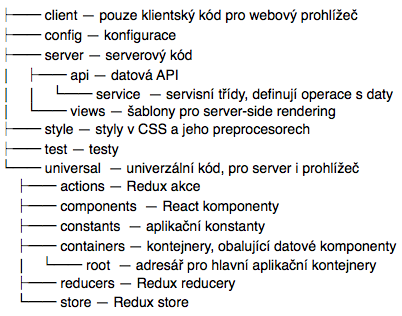
\includegraphics[scale=0.6]{obrazky/struktura}
\par\end{centering}
\caption{Adresářová struktura ukázkové webové aplikace \label{fig:structure}}
\end{figure}
\FloatBarrier
          
\subsection{Vstupní body aplikace}              
Ukázková aplikace obsahuje dva vstupní body, tedy soubory ze kterých je spuštěna inicializace webové aplikace. Každý z nich je určený pro odlišné prostředí, jeden pro server a druhý po prohlížeč. Oba dva v podstatě spouští totožnou aplikaci, ale při použití isomorfního přístupu je jejich použití nezbytné. Jedná se o soubory:
\begin{itemize}
\item \textbf{server.js} – nastartuje webový server v node.js, který zpracovává HTTP požadavky na API a spouští serverové vykreslování požadované šablony.
\item \textbf{client/app.js} – spustí se v prohlížeči při prvním načtení webové aplikace, pokud je povolený Javascript. Aplikace si načte prvotní stav předaný serverem a spustí celou klientskou část aplikace, ta je po kompletním načtení plně zodpovědná za další obsluhu.
\end{itemize} 

\subsection{Sdílený kód}
Isomorfní kód, neboli univerzální Javascript je uložen v adresáři \textit{universal}. Ten obsahuje definici routování, všechny React komponenty nebo kompletní definici obsluhy dat dle architektury Flux. Tu v naší ukázkové aplikaci realizuje nástroj Redux, jehož komponenty jsou uloženy ve složkách \textit{actions}, \textit{reducers} a \textit{store}. Komponenty uživatelského rozhraní jsou v aplikaci dvou typů. Tím prvním jsou klasické React komponenty, zobrazující nějaká data, nebo reprezentující společné části HTML layoutu. Ty jsou uloženy v adresáři \textit{components}. Druhý typ jsou takzvané \uv{kontejnerové komponenty}. Ty v kontextu frameworku React většinou tvoří jednak samotnou webovou aplikaci (hlavní komponenta) nebo se používají pro zobrazování kolekcí. Kontejnery používají vlastní složku \textit{containers}. Poslední důležitou části sdíleného kódu jsou routovací pravidla, ty jsou definována pomocí JSX pro nástroj React-router a uložena v souboru \textit{routes.js}. Tento soubor také importuje serverová část aplikace, kvůli nutnosti routování požadavků také na serveru.

\subsection{Serverová část}
Serverová část aplikace využívá framework Express a řeší vedle datového API také vykreslování samotné React aplikace, respektive ve většině případů jenom jejího prvotního stavu. Je definována v souboru server.js v kořenovém adresáři aplikace.
\begin{lstlisting}[language=Javascript, caption={Ukázka serverové části isomorfní webové aplikace}]
// servírování statického obsahu (obrázky, CSS, apod.)
app.use(require('serve-static')(path.join(__dirname, config.get('buildDirectory'))));

// definice API
app.get('/api/0/events', api.getEvents);
app.post('/api/0/events', api.addEvent);
app.post('/api/0/events/:id', api.editEvent);
app.delete('/api/0/events/:id', api.deleteEvent);

// favicon
app.get('/favicon.ico', (req, res) => res.sendFile(path.join(__dirname, 'images', 'favicon.ico')));

// definice metody pro serverove vykreslovani
app.get('*', uni.handleRender);
\end{lstlisting}

Syntaxe je velmi jednoduchá, nad Express objektem app existují funkce \textit{get}, \textit{post} a další, které reprezentují jednotlivé HTTP metody. Ty vždy přijímají dva argumenty, URL na kterém naslouchají a obslužnou funkci, které HTTP požadavek předají. Příklad ilustruje definici API, nastavení servírování statických souborů a hlavně také isomorfní server-side rendering. Ten provádí funkce \textit{handleRender()}. Ta provede na jakékoliv URL, které neodpovídají jiné definice, serverové vykreslení celé isomorfní webové aplikace. Tato funkce vyhodnotí URL a za základě routovacích pravidel získaných ze sdíleného kódu, vykreslí celou javascriptovou aplikaci na serveru a vrátí zpracované HTML, které poté klientská část načte a celou webovou aplikaci spustí v prohlížeči.
\subsection{Klientská část}
Klientskou část tvoří standardní React aplikace v Javascriptu. Její spuštění ilustruje tato ukázka kódu.
\begin{lstlisting}[language=Javascript, caption={Ukázka klientské části isomorfní webové aplikace}]
import routes from '../universal/routes';
import store from '../universal/store';
import * as actions from '../universal/actions/GuestbookActions';

import Root from '../universal/containers/root';

import '../style/pure.css';
import '../style/main.styl';
import '../style/spinner.styl';

const history = syncHistoryWithStore(browserHistory, store);

ReactDOM.render(
  <Root store={store} routing={routes} history={history} />,
  document.getElementById('app')
);
\end{lstlisting}

Využívá se universální kořenová Root komponenta, která přijímá Redux store, a instanci React routeru. Na základě předaných routovacích pravidel a aktuální URL dojde k vykreslení související kontejnerové komponenty. Zajímavosti je definice stylů pomocí příkazu \textit{import}, a to jak samotného CSS tak i stylopisů využívající preprocesor Stylus. O jejich načtení a zkompilování se postará module bundler webpack.

\begin{lstlisting}[language=Javascript, caption={Ukázka implementace kořenové React komponenty}]
export default class Root extends Component {
  render() {
    const { store, routing, history } = this.props;
    return (
      <Provider store={store}>
        <div>
          <Router history={history}>
            {routing}
          </Router>
        </div>
      </Provider>
    );
  }
};
\end{lstlisting}

\subsection{Testy}
Testy jsou v ukázkové aplikaci uloženy v adresáři \textit{test}. Jsou implementovány testy akcí a reducerů nástroje Redux. Při testování akcí ověřujeme, zda volání nějaké metody vytvoří správné Redux akce se správnými atributy. Testování reducerů má zase za úkol ověřit správnost mutace aplikačního stavu, jehož změny mají reducery na starost. Následuje ukázka jednoduchého testu akcí při získávání komentářů z API. Test kontroluje vznik akcí \textit{LOAD\_COMMENTS\_REQUEST} a \textit{LOAD\_COMMENTS\_SUCCESS} s příslušnou strukturou.
\begin{lstlisting}[language=Javascript, caption={Ukázka asynchronního testu získávání datových entit – komentářů}]
  describe('loadComments', () => {
    const mockStore = configureStore([thunk]);
    it('should trigger a LOAD_COMMENTS_REQUEST and LOAD_COMMENTS_SUCCESS action when succesful', () => {
      let requestMock = {
        get: () => ({
          set: () => ({
            end: (x) => x(null, {
              body: [ { name: 'Awesome', author: 'John Doe' } ]
            })
          })
        })
      };
      actions.__Rewire__('request', requestMock);
      let expectedActions = [
        { type: 'LOAD_COMMENTS_REQUEST' },
        { type: 'LOAD_COMMENTS_SUCCESS', events: [ { name: 'Awesome', author: 'John Doe' } ] }
      ];
      
      let initialState = {guestbookApp: { comments: [], userId: 'baseUser'} };
      let store = mockStore(initialState);

      store.dispatch(loadComments());
      const actualActions = store.getActions();
      expect(actualActions).to.eql(expectedActions);
    });
\end{lstlisting}


\chapter{Porovnání s existujícími vývojovými postupy}
Isomorfní přístup k programování webových aplikací je relativně nový princip, který přináší použití Javascriptu pro webový prohlížeč i webový server. Použití jednoho jazyka pro obě prostředí přináší mnoho výhod, je možné vyvíjet veškerý kód v jednom projektu, používat stejné knihovny nebo dokonce sdílet kód mezi jednotlivými prostředími. Nejdůležitější technologií, která isomorfní přístup umožnila, bylo bezesporu node.js. To přineslo možnost zpracovávat Javascript také na serveru. Využití Javascriptu na serveru také řeší většinu problémů jednostránkových aplikací, použití isomorfního přístupu je tedy ideální při vývoji velmi interaktivní aplikace. Je všeobecně známo, že jsou běžné jednostránkové aplikace nevhodné pro vývoj webu, kde je nezbytná dobrá indexovatelnost internetovými vyhledávači. Obecně se proto nedoporučuje programovat jako SPA obsahově založené weby, například magazíny nebo blogy. Použití isomorfního Javascriptu tento problém řeší a umožňuje tak naprogramovat jako SPA jakýkoliv web. Následující dva diagramy dobře ilustrují rozdíly v architektuře klasických a isomorfních jednostránkových webových aplikací.

\vspace{0,3cm}
\begin{figure}[h]
\begin{centering}
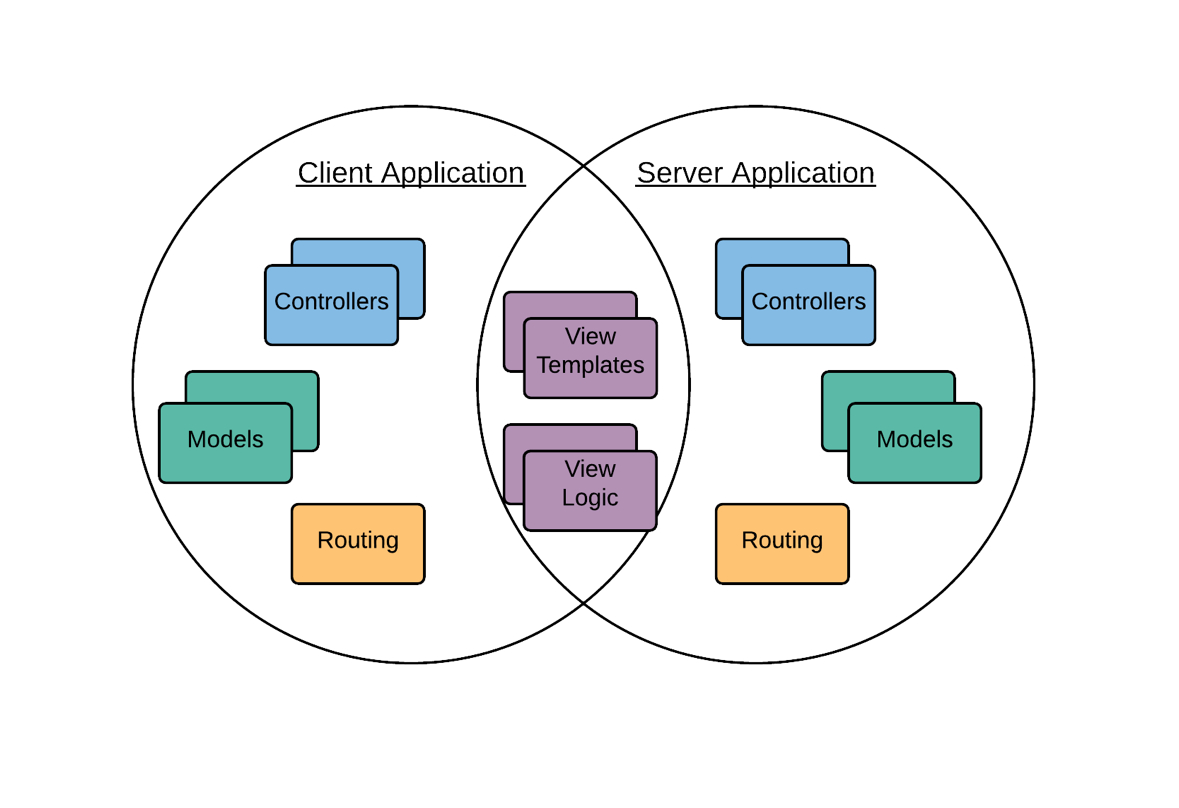
\includegraphics[scale=0.4]{obrazky/sharing_view}
\par\end{centering}
\caption{Diagram archiktuktury běžné jednostránkové aplikace \cite{isomorhic_book} \label{fig:spa_arch}}
\end{figure}

Běžné jednostránkové webové aplikace striktně oddělují serverovou a klientskou část aplikace. V době jejich vzniku to bylo považováno za výhodu, protože takové rozdělení aplikace zjednodušuje vývoj a umožňuje snadno vytvářet další klienty, například mobilní aplikace. Časem se však projevily problémy a nedostatky tohoto řešení. Koncept isomorfních aplikací proto opět spojuje serverovou a klientskou část a díky použití stejného jazyka umožňuje také sdílení kódu.

\begin{figure}[h]
\begin{centering}
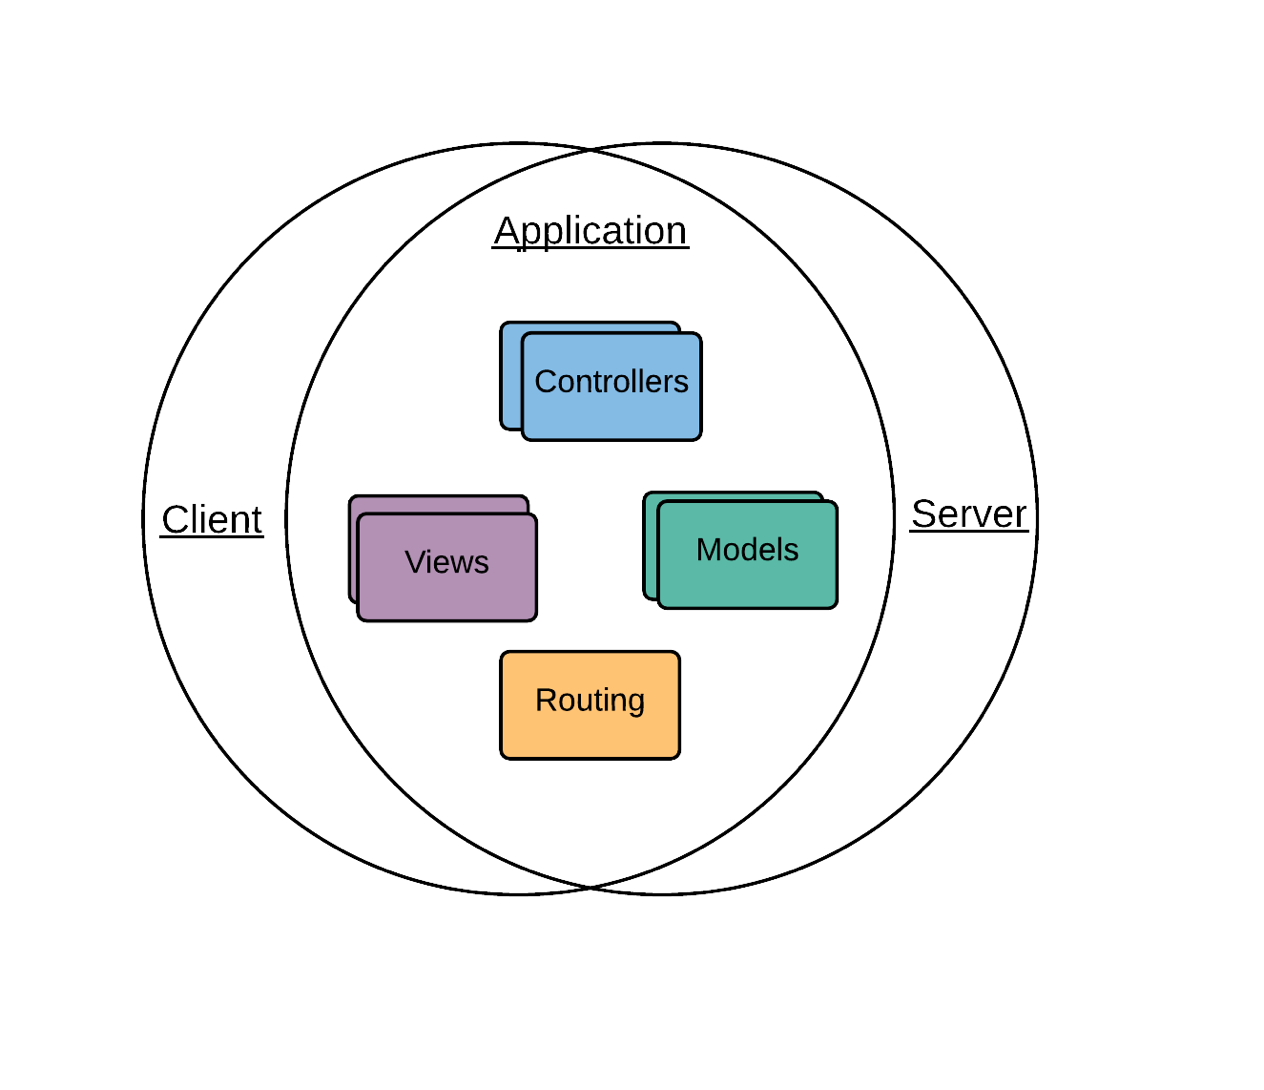
\includegraphics[scale=0.4]{obrazky/sharing_all}
\par\end{centering}
\caption{Diagram architektury isomorfní webové aplikace \label{fig:isomorphic_arch}}
\end{figure}
\FloatBarrier

Isomorfní webové aplikace sdílejí základní programové komponenty mezi serverem a prohlížečem. To je možné jen při použití stejného jazyka pro obě prostředí, kterým dnes může být jen Javascript. Isomorfní přístup konečně přináší plně indexovatelné jednostránkové webové aplikace. Porovnáme-li složitost implementace isomorfní aplikace s běžnou SPA, napsanou například v AngularJS, zjistíme, že se velmi liší. Je to dáno především specifickou syntaxí AngularJS a na druhé straně použitím jiných přístupů a nové syntaxe ES6 v React. Programátor je tak nucen osvojit si některé zcela nové přístupy, jinou syntaxi a některé specifické návrhové vzory. Jejich použití je ale dnes již do značné míry standardizované, můžeme tedy očekávat, že se budou v Javascriptu používat i za několik let. 

Eric Mathiason se ve své práci mimo jiné zaměřil na porovnání knihoven vhodných pro isomorfní přístup s klasickými SPA frameworky. Jeho práce porovnává frameworky React a Ember.js. Ember byl vybrán především proto, že není tolik komplexní jako například Angular, a tak se lépe hodí pro srovnání s React, který řeší především obsluhu uživatelského rozhraní. Následující tabulka shrnuje vlastnosti těchto frameworků \cite{mathiasson-isomorphic}.
\begin{table}[h]
\centering
	\caption{Srovnání javascriptových frameworků React a Ember.js \cite{mathiasson-isomorphic}}
	\begin{tabular}{ |p{6.5cm}|C{1.5cm}|C{1.5cm}| }
	\hline
	& React & Ember.js \\ \hline
	Podpora pro implementaci SPA & ANO & ANO \\ \hline
	Možnost serverového vykreslování & ANO & NE \\ \hline
	Použití vlastního šablonovacího jazyka & ANO & ANO \\ \hline
	Nízký průměrný čas načítání & ANO & NE \\ \hline
	REST komunikace & ANO & ANO \\ \hline
	Jednosměrný tok dat & ANO & NE \\ \hline
    \end{tabular}
	\label{tab:react_vs_ember}
\end{table}
\FloatBarrier

Mathiason se také zaměřil na srovnání rychlosti vykreslování javascriptové aplikace využívájící React a Ember.js. V tomto testu nebylo využito serverové vykreslování, které by dobu načítání React aplikace ještě snížilo \cite{mathiasson-isomorphic}.

\begin{figure}[h]
\begin{centering}
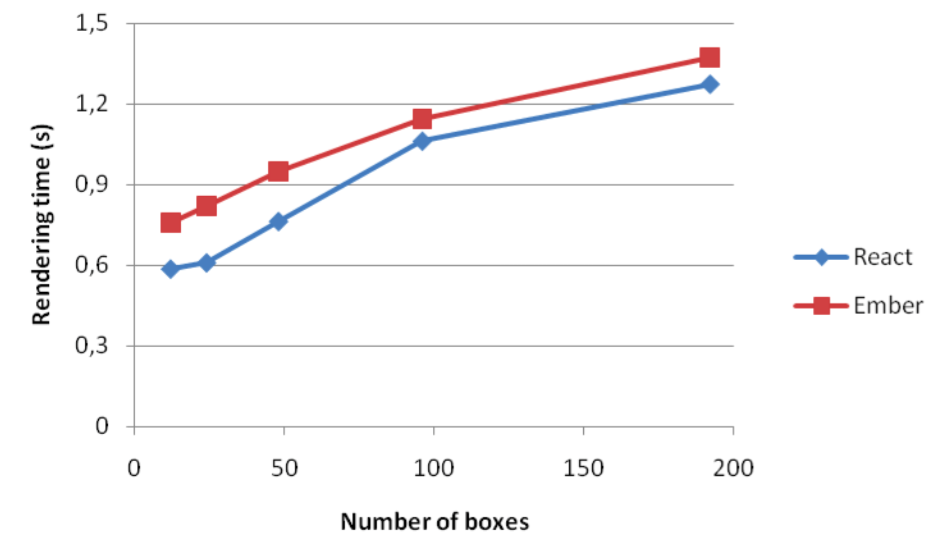
\includegraphics[scale=0.4]{obrazky/comparison_1}
\par\end{centering}
\caption{Porovnání rychlostí vykreslování frameworků React a Ember.js \cite{mathiasson-isomorphic} \label{fig:comparison_2}}
\end{figure}
\FloatBarrier

Porovnat isomorfní aplikace s klasickými serverově orientovanými frameworky, který používají Javascript jen okrajově, je složité. Především proto, že chování čistě serverové aplikace je značně odlišné od chování aplikace založené na Javascriptu. Serverové aplikace například neposkytují takovou interaktivitu jakou obecně jednostránkové aplikace nabízejí. Implementace vysoce dynamických aplikací ale bývá složitější především kvůli některým vlastnostem jazyka Javascript. Určitou zvláštností javascriptového vývoje je také používání velkého množství knihoven a z toho vycházející nutnost jejich konfigurace, která může být často složitá. V tomto prostředí začíná klesat popularita ucelených frameworků, na úkor velmi modulárních řešení, poskládaných z mnoha malých knihoven. Místo výrazu framework se v Javascriptu dnes často používá pojem \textit{devstack}. Jedná se o připravený soubor knihoven, tvořící kompletní vývojové prostředí. Dobře nakonfigurovaný devstack potom zastává funkce velkého monolitického frameworku známého z ostatních programovacích jazyků. Navíc však myslí i na pohodlí vývojáře. Devstacky pro vývoj isomorfních webových aplikací často podporují \textit{hot reloading}, což znamená okamžité doručování aktuální verze zdrojového kódu do webového prohlížeče. Každá změna ve zdrojovém kódu se okamžitě projeví v prohlížeči. Okamžitá propagace změn je velkým specifikem isomorfního přístupu. V jiných jazycích je nutné vyvíjené aplikace často restartovat, Javascript lze díky jeho návrhu modifikovat za běhu, nutnost restartování webové aplikace tedy odpadá a díky nástrojům jako Webpack, nemusí vývojář provádět ani obnovení samotné webové stránky ve webovém prohlížeči \cite{webpack}.

\chapter{Výsledky}
Práce si kladla za cíl především představit isomorfní přístup jako vhodnou techniku pro programování moderních webových aplikací. Tento přístup byl také porovnán s jinými zažitými principy vývoje. Isomorfní webové aplikace jsou v podstatě dalším evolučním stupněm vývoje jednostránkových webových aplikací v jazyce Javascript. Oproti klasickým jednostránkovým webovým aplikacím, které běží kompletně v prohlížeči, je implementace isomorfní aplikace o něco málo náročnější. Při použití vhodných nástrojů, které jsou navrženy pro běh v prohlížeči nebo node.js, je složitost vývoje isomorfních aplikací srovnatelná s běžnými SPA. Implementace klasických serverově orientovaných aplikací je samozřejmě jednodušší, především díky zažitým komplexním frameworkům a mnoha příkladům, které jejich vývoj velmi usnadňují. V poslední době ale popularita čistě serverových aplikací stále klesá. Vysoká interaktivita bývá základním požadavkem čím dál tím více webových aplikací, proto se stává isomorfní přístup stále populárnější. Jeho použití se vyplatí pro většinu typů aplikací, velmi totiž vylepšuje výslednou uživatelskou přívětivost aplikace a díky obnovování jen určitých částí stránky, také její intuitivnost. Určitou komplikací vývoje moderních webových aplikací v Javascriptu je velká dynamičnost vývoje používaných knihoven. Často vycházejí nové verze, přinášející mnoho změn, některé z nich mohou být také \textit{breaking changes}, tedy takové změny, které nejsou kompatibilní se starší verzí dané knihovny. To je dáno především tím, že většina knihoven určených pro isomorfní vývoj je stará pouze několik let a celé jejich rozhraní tak ještě není ustáleno. Řešením je definice přesných verzí knihoven v souboru \textit{package.json} a větší opatrnost při jejich upgradování.

Využití isomorfního přístupu je v podstatě nezbytné, tvoří-li programátor obsahově založenou webovou stránku, například zpravodajský server, diskuzní fórum, nebo jakoukoliv jinou webovou aplikaci, ke které se přistupuje převážně z internetového vyhledávače. Alespoň některý její obsah tedy má být veřejný. Jako klasické SPA se často vyvíjejí uzavřené informační systémy, kde se jejich nevýhody prakticky neprojevují. Tyto systémy totiž většinou vyžadují přihlášení a jejich obsah nemá být veřejně dostupný. I pro ně je ale isomorfní přístup vhodný a vzhledem k tomu, že celý přístup je fakticky evolucí vývoje v Javascriptu, lze očekávat že se jeho pomocí budou vytvářet všechny webové aplikace v Javascriptu. V současnosti jsou nejpoužívanější vývojové nástroje od společnosti Facebook, které z nich se ale nakonec stanou standardem, ukáže až čas.

Praktickým výsledkem této diplomové práce je ukázková isomorfní webová aplikace, na které jsou demonstrovány popisované přístupy. Vytvořená aplikace funguje ve většině internetových prohlížečů na běžném počítači, mobilním telefonu nebo tabletu. Aplikace je přínosná tím, že ukazuje moderní postupy při tvorbě interaktivních webových aplikací. Přínosem práce je také to, že se jedná o první akademickou práci zabývající se vývojem isomorfních webových aplikací vydanou v České republice.